\documentclass{article}\usepackage[]{graphicx}\usepackage[]{xcolor}
% maxwidth is the original width if it is less than linewidth
% otherwise use linewidth (to make sure the graphics do not exceed the margin)
\makeatletter
\def\maxwidth{ %
  \ifdim\Gin@nat@width>\linewidth
    \linewidth
  \else
    \Gin@nat@width
  \fi
}
\makeatother

\definecolor{fgcolor}{rgb}{0.345, 0.345, 0.345}
\newcommand{\hlnum}[1]{\textcolor[rgb]{0.686,0.059,0.569}{#1}}%
\newcommand{\hlsng}[1]{\textcolor[rgb]{0.192,0.494,0.8}{#1}}%
\newcommand{\hlcom}[1]{\textcolor[rgb]{0.678,0.584,0.686}{\textit{#1}}}%
\newcommand{\hlopt}[1]{\textcolor[rgb]{0,0,0}{#1}}%
\newcommand{\hldef}[1]{\textcolor[rgb]{0.345,0.345,0.345}{#1}}%
\newcommand{\hlkwa}[1]{\textcolor[rgb]{0.161,0.373,0.58}{\textbf{#1}}}%
\newcommand{\hlkwb}[1]{\textcolor[rgb]{0.69,0.353,0.396}{#1}}%
\newcommand{\hlkwc}[1]{\textcolor[rgb]{0.333,0.667,0.333}{#1}}%
\newcommand{\hlkwd}[1]{\textcolor[rgb]{0.737,0.353,0.396}{\textbf{#1}}}%
\let\hlipl\hlkwb

\usepackage{framed}
\makeatletter
\newenvironment{kframe}{%
 \def\at@end@of@kframe{}%
 \ifinner\ifhmode%
  \def\at@end@of@kframe{\end{minipage}}%
  \begin{minipage}{\columnwidth}%
 \fi\fi%
 \def\FrameCommand##1{\hskip\@totalleftmargin \hskip-\fboxsep
 \colorbox{shadecolor}{##1}\hskip-\fboxsep
     % There is no \\@totalrightmargin, so:
     \hskip-\linewidth \hskip-\@totalleftmargin \hskip\columnwidth}%
 \MakeFramed {\advance\hsize-\width
   \@totalleftmargin\z@ \linewidth\hsize
   \@setminipage}}%
 {\par\unskip\endMakeFramed%
 \at@end@of@kframe}
\makeatother

\definecolor{shadecolor}{rgb}{.97, .97, .97}
\definecolor{messagecolor}{rgb}{0, 0, 0}
\definecolor{warningcolor}{rgb}{1, 0, 1}
\definecolor{errorcolor}{rgb}{1, 0, 0}
\newenvironment{knitrout}{}{} % an empty environment to be redefined in TeX

\usepackage{alltt}
\title{Decision Tree Modeling of Frog Species}
\author{Alex Hey}
\date{\today}
\IfFileExists{upquote.sty}{\usepackage{upquote}}{}
\begin{document}
\maketitle

\section{Introduction}
In this toy analysis, we applied various machine learning models to classify frog species based on MFCC data. This report presents the results of decision tree models trained on a subset of the data and evaluates their performance.

\section{Methods}
\subsection{Data Preparation}
The dataset, \texttt{Frogs\_MFCCs.csv}, was split into a training set and a test set with a 75-25 ratio. 

\subsection{Model Training}
We trained decision trees with and without pruning. A k-fold cross-validation was performed using the \texttt{caret} package to assess model performance.

\section{Results}
\subsection{Error Rates}
The error rates for each model variant are summarized in Table~\ref{tab:results}. Based on these results, we observed that the unpruned tree performed slightly better than the pruned tree.

% latex table generated in R 4.3.2 by xtable 1.8-4 package
% Fri Nov 15 23:35:31 2024
\begin{table}[ht]
\centering
\begin{tabular}{lr}
  \hline
Method & ErrorRate \\ 
  \hline
Unpruned Tree (Train) & 0.00 \\ 
  Unpruned Tree (Test) & 0.01 \\ 
  Pruned Tree (Train) & 0.00 \\ 
  Pruned Tree (Test) & 0.01 \\ 
  Cross-Validated Tree & 0.29 \\ 
   \hline
\end{tabular}
\caption{Error rates for different model variants} 
\label{tab:results}
\end{table}


\subsection{Figures and Tables}
Figure~\ref{fig:tree} shows the structure of the final decision tree model. 

\begin{figure}[h]
    \centering
    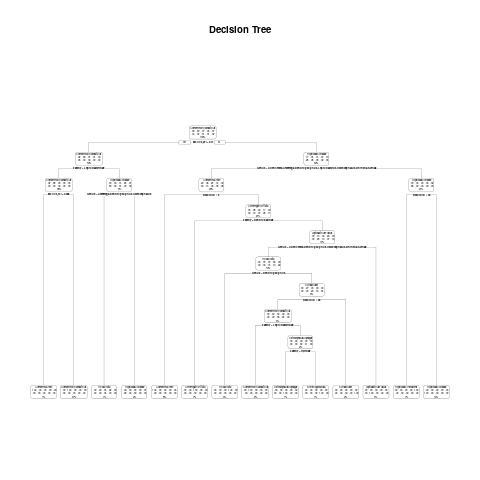
\includegraphics[width=0.6\textwidth]{../results/decision_tree.png}
    \caption{Decision Tree structure used for classification of frog species.}
    \label{fig:tree}
\end{figure}

\section{Supplementary Information}
For additional details, refer to the Supplementary Information (SI) file~\cite{Reuman2024}. I made up a random citation just to get practice with it. 

\section{Conclusion}
I'm trying out new formats and sections here.

\bibliographystyle{plain}
\bibliography{references}

\end{document}
